\documentclass[iicol,pdflatex,sn-basic,Numbered]{sn-jnl}

\usepackage{graphicx}
\usepackage{booktabs}
\usepackage{multirow}
\usepackage{amsmath}
\usepackage{amssymb}
\usepackage{xurl}

\newcommand{\asds}{\mathrm{ASDS}}

\begin{document}

\title[Reference-conditioned Chinese calligraphy assessment]
{Reference-Conditioned Structural Assessment of Low-Resource Chinese
Calligraphy with Overlapping Stroke Parsing and Human-Audited Spatial
Scoring}

\author*[1]{\fnm{Xiaofan} \sur{Liu}}
\email{10244602411@stu.ecnu.edu.cn}
\equalcont{These authors contributed equally to this work.}
\author[1]{\fnm{Ronghao} \sur{Zhang}}
\equalcont{These authors contributed equally to this work.}
\author[1]{\fnm{Yuan} \sur{Feng}}
\equalcont{These authors contributed equally to this work.}
\affil*[1]{\orgdiv{School of Software Engineering},
  \orgname{East China Normal University},
  \orgaddress{\city{Shanghai}, \country{China}}}

\abstract{%
\textbf{Purpose:} Computer-vision systems for handwriting commonly assume
mutually exclusive semantic regions, optimize recognition or style
classification, or compare images without separating global placement from
local structural error. None returns what assessing a handwritten Chinese
character against a same-character reference requires: two instances can be
equally recognizable yet differ in the local stroke structure a learner
should revise. We formulate reference-conditioned structural assessment as
an auditable document-analysis problem under limited labelled data.
\par
\textbf{Methods:} An overlapping six-channel parser predicts five
independently activated direction masks and an endpoint mask; U-Net,
DeepLabV3+, and SegFormer-B2 are compared with three seeds on standard and
character-disjoint splits of 769 quality-controlled samples. Constrained
similarity registration, three structural scores, and localized diagnostic
evidence are evaluated on 200 references under controlled perturbations and
on 150 natural pairs rated blindly by three calligraphy-domain raters, two of
them authors.
\par
\textbf{Results:} DeepLabV3+ reaches \(0.9630\pm0.0006\) standard-split
Macro Dice, SegFormer-B2 leads character-disjoint direction parsing at
\(0.8866\pm0.0008\), and U-Net leads strict endpoint F1. Registration
reduces nuisance penalties by 30.118 points relative to no alignment on
clipping-safe cases while preserving 11.189 additional points of structural
penalty. The frozen production score, a coverage-aware score, and a
retrospectively developed aligned spatial-distribution similarity (ASDS)
reach Spearman correlations of 0.297, 0.429, and 0.556;
character-grouped out-of-fold ASDS retains 0.540, and direct-ink ASDS is
nearly equivalent (\(\Delta\rho=0.0004\)), so direction-level evidence, not
the scalar, justifies the parser. Localized evidence reaches Recall@3 of
0.701 but exact-cell localization of 0.109.
\par
\textbf{Conclusion:} We deliver a reproducible framework for overlapping
parsing, discrepancy-preserving registration, and human-audited localized
feedback.}

\keywords{Chinese calligraphy, document analysis, multi-label segmentation,
reference-based assessment, human validation, explainable feedback}

\maketitle

\section{Introduction}
\label{sec:introduction}

Calligraphy---the writing of Chinese characters with a brush---is a
foundational form of traditional Chinese culture. Its principal script styles,
seal (\emph{zhuan}), clerical (\emph{li}), regular (\emph{kai}), running
(\emph{xing}), and cursive (\emph{cao}), employ distinct stroke techniques and
convey a wide range of qualities, from dignified and elegant to vigorous,
unrestrained, archaic, and lively. Two handwritten instances of the same
Chinese character can be equally
legible yet differ in the local structure relevant to calligraphy
(\emph{shufa}) instruction. A teacher may identify a shortened horizontal
stroke, a displaced hook, a low component, or an endpoint that fails to meet
its neighbour. Figure~\ref{fig:pipeline}(a) illustrates structural differences
using a regular-script reference and a running-script candidate of the same
character. Both are recognizable, but their stroke proportions, junctions,
and component spacing differ. These cross-style differences illustrate the
comparison task; they do not establish that either instance is incorrect.
Useful feedback must identify the relevant discrepancies and their locations
relative to the selected reference.

Global placement can vary without changing the local structure being
assessed. A character may be slightly larger, shifted on the canvas, or
tilted by a degree or two. Missing terminal fragments, over-wide strokes,
and misproportioned components should remain visible after such differences
are compensated. Reference-conditioned assessment must therefore separate
global placement from local discrepancy and return inspectable evidence
alongside a scalar score.

Recognition, style classification, and generation address character
identity, style category, and glyph synthesis, respectively
\cite{liu2013casia,zhang2026callinet,xu2026unicalli}. These objectives do not
directly evaluate spatially resolved, direction-specific discrepancies
between two instances. Formulating same-character structural comparison as
a document-analysis task exposes four computer-vision challenges.
\begin{enumerate}
  \item[C1] \emph{Overlapping labels under scarce annotation.} At crossings
  and adhesions, a pixel can carry multiple direction labels, which a
  mutually exclusive partition cannot represent. Endpoint evidence is sparse,
  and dense annotation is limited to 769 quality-controlled observations of
  40 character identities, without reliable writer identities.
  \item[C2] \emph{Global nuisance versus local structure.} Direct overlap
  confounds structure with translation, scale, and rotation. Flexible
  registration can erase proportion or component-placement errors, while an
  overlap score can reward direction channels that are empty in both images.
  \item[C3] \emph{Stability is not validity.} A score that is stable under
  allowed transforms may still disagree with how trained readers perceive
  structural similarity.
  \item[C4] \emph{A scalar does not localize.} Feedback must identify the
  direction family, the affected region, and whether ink is missing or extra.
  Fluent text cannot make an incorrect structural attribution reliable.
\end{enumerate}

\begin{figure*}[!t]
  \centering
  
\includegraphics[width=\textwidth]{figures/redrawn/figure1_pipeline.pdf}
  \caption{Reference-conditioned structural assessment on one same-character
  pair. (a)~A regular-script reference and a running-script candidate of the
  same character are recognizable but structurally different. (b)~The candidate
  is parsed into overlapping direction channels vec1--vec5; the reference
  follows the same procedure. Black pixels carry multiple direction labels,
  and cyan outlines mark endpoints. The framed inset shows the multi-label
  bounding box at reduced scale. (c)~A bounded global transform registers the
  reference to the candidate, compensating global size and tilt (here scale
  1.20 and rotation \(3^\circ\)). The residual comprises overlap (dark grey),
  missing reference ink (blue, hatched), and extra candidate ink (red,
  counter-hatched). (d)~The aligned silhouette on the
  \(3\times3\) grid used for localized evidence; the values beneath it are
  the three ASDS spatial-distribution similarities of
  Sect.~\ref{sec:scores}. (e)~The structured output includes the production
  score, weakest direction family and its Dice, ink IoU, endpoint F1,
  transform, and missing/extra regions. The reported direction Dice belongs
  to that family, rather than the five-channel mean. All evidence is
  available before text generation. The cross-style pair is illustrative;
  the human study uses
  natural same-character, different-instance pairs from the project corpus. Source images: Calli-Tongji open subset \cite{yunmo_jixin_2025},
  CC~BY-NC~4.0.}
  \label{fig:pipeline}
\end{figure*}

Figure~\ref{fig:pipeline} outlines the framework, from overlapping structural
parsing and bounded registration to scalar agreement and localized evidence.
Parsing addresses C1, while registration and the score-semantics audit
address C2. The human study and diagnostic benchmark evaluate C3 and C4,
respectively, through the following research questions.
\begin{description}
  \item[RQ1 (representation and generalization).] Can convolutional and
  transformer parsers trained on the quality-controlled corpus of
  Sect.~\ref{sec:data} recover overlapping direction masks and sparse
  endpoint masks? How much does performance decline for character identities
  absent from training?
  \item[RQ2 (registration and score behaviour).] Relative to no alignment,
  does a constrained similarity registration reduce sensitivity to nuisance
  transforms while preserving penalties for controlled structural changes?
  Does a wider search improve this trade-off? How do channel-coverage
  semantics affect the frozen score, and does it distinguish same-character
  pairs on real references?
  \item[RQ3 (human validity).] How strongly do the frozen production score,
  the coverage-aware score, and aligned spatial-distribution similarity
  (ASDS) associate with blinded ratings of same-character structural
  similarity? Does the ASDS scalar depend on six-channel parsing?
  \item[RQ4 (localized diagnosis).] Which localized diagnostic outputs are
  reliable on interventions with known ground truth, and why do they fail?
\end{description}

The study makes four contributions aligned with these research questions.
\begin{enumerate}
  \item For RQ1, we define five independently activated direction-family
  channels and an endpoint channel, without a per-character prior at
  inference. The representation differs from Stroke-Seg's stroke instances
  (Sect.~\ref{sec:related}). Semantic quality control supports a matched
  three-seed comparison of U-Net, DeepLabV3+, and SegFormer-B2 on standard
  and character-disjoint splits. Ranking depends on
  target and protocol: DeepLabV3+ leads in-corpus direction parsing,
  SegFormer-B2 unseen-character direction parsing, and U-Net strict endpoint
  localization.
  \item For RQ2, we evaluate constrained similarity registration using
  controlled nuisance and structural perturbations of 200 real references.
  Paired comparisons cover no alignment and the tested wider, coarser search, alongside an
  inactive-channel score audit. Constrained registration
  substantially reduces nuisance penalties relative to no alignment, while
  structural edits remain penalized. Residual sensitivity and clipping-conditional
  summaries delimit this result.
  \item For RQ3, we compare the three scores in a blinded three-rater study
  and add a paired direct-ink control. ASDS development is retrospective,
  with character-grouped internal validation. Its observed association is
  strongest, but the direct-ink control supports a silhouette interpretation;
  direction-level evidence provides the rationale for the parser.
  \item For RQ4, we evaluate localized structured evidence and classify its
  failures. Required findings are usually surfaced, but exact-cell
  localization remains unreliable because of multi-cell truth and direction
  attribution errors. Language generation remains downstream of the
  structured evidence.
\end{enumerate}

The intended input is a raster exported from a direct digital writing canvas,
not a photograph. The claims concern reference-conditioned structural
analysis in this modality. They do not extend to camera robustness, writer-disjoint generalization,
stroke-order recovery, historical authenticity, or universal aesthetic
grading.

\section{Related Work}
\label{sec:related}

\subsection{Recognition, document segmentation, and stroke parsing}

Large databases such as CASIA-HWDB established benchmarks for online and
offline handwritten Chinese character recognition \cite{liu2013casia}.
Recognition assigns character identities; assessing local structure
additionally requires spatially resolved outputs. Dense prediction provides
a basis for representing the regions that compose a document image.
U-Net introduced an encoder--decoder with skip connections
\cite{ronneberger2015unet};
DeepLabV3+ combines atrous spatial pyramids with a decoder
\cite{chen2018deeplabv3plus}; and SegFormer pairs hierarchical transformer
features with a lightweight multilayer-perceptron decoder
\cite{xie2021segformer}. In document analysis, dhSegment showed that one generic
segmentation formulation can serve many page-level tasks
\cite{oliveira2018dhsegment}. A recent IJDAR study found that label
scarcity, source--target mismatch, and pretraining protocol affect handwritten
document segmentation \cite{baloun2025selfsupervision}. Standard semantic segmentation assigns
each pixel one class \cite{chen2018deeplabv3plus,xie2021segformer}.

Stroke-Seg addresses stroke-level analysis through a multi-label framework
compatible with several segmentation backbones \cite{gong2024strokeseg}.
Its output assigns intersection pixels to multiple strokes, and a prior
vector supplies character-specific stroke-composition information. The
framework is evaluated by true stroke rate on a brush-calligraphy
stroke-segmentation dataset \cite{gong2024strokeseg}.

\subsection{Computational calligraphy and handwriting-quality evaluation}

Early computational calligraphy work represented style with local and
global shape features
\cite{zhang2015calligraphic,gao2017calligraphic}; CalliNet advances style
classification with metric learning and triplet supervision
\cite{zhang2026callinet}. Other systems extract artistic regions relative
to a reference image \cite{wang2018artistic} or beautify handwritten glyphs
toward a Kai-style template \cite{xia2009beautification}. Designed aesthetic
features have also been used to evaluate robotic writing
\cite{ma2017aesthetics}. Large recent resources such as
UniCalli support column-level generation and recognition
\cite{xu2026unicalli}.

A survey groups handwritten Chinese character quality evaluation into
rule-based geometric measures, template comparison, and learned methods
\cite{chen2024qualitysurvey}. Defining quality labels and explaining model
decisions remain open problems \cite{chen2024qualitysurvey}. Siamese networks learn pairwise quality from
labelled examples \cite{chen2025siamhcc}, and a recent shared task combined
writing-quality grading with comment generation on an expert-annotated
dataset \cite{liu2025calligraphyeval}. Across these studies, quality spans
several constructs, including legibility, geometric correctness, reference
similarity, brushwork, and artistic appeal. These constructs can disagree,
making the assessment target consequential for its interpretation.

\subsection{Registration, shape description, and human validation}

Image registration ranges from parametric geometric alignment to learned
spatial transformers \cite{zitova2003registration,jaderberg2015stn}.
Registration surveys distinguish rigid, similarity, and affine models from
elastic and deformable models by the shape differences they can absorb
\cite{zitova2003registration}. Shape contexts describe the
spatial distribution of contour points in log-polar bins
\cite{belongie2002shapecontext}, and spatial pyramids retain coarse layout
that an orderless representation would discard
\cite{lazebnik2006spatialpyramid}. Distributions of this kind can be compared
with the bounded, symmetric Jensen--Shannon divergence \cite{lin1991jensen}.

Assessment against human judgment requires both a measure of association
and an account of rater reliability. Two-way random-effects,
absolute-agreement intraclass correlations quantify agreement among raters
\cite{mcgraw1996icc,koo2016icc}, while bootstrap resampling estimates
uncertainty in score--rating associations
\cite{efron1993bootstrap}.

\section{Data Resources}
\label{sec:data}

The experiments use a project corpus with manual ground truth (GT), an
external reference library, and a human-rating cohort selected from the
quality-controlled (QC) project corpus. Table~\ref{tab:cohorts} distinguishes
their annotation sources and the research questions they support.

\begin{table*}[t]
\caption{Data resources, their label status, and the research question (RQ)
each serves. GT denotes manual six-channel ground truth.}
\label{tab:cohorts}
\centering
\scriptsize
\setlength{\tabcolsep}{4pt}
\begin{tabular}{@{}p{2.6cm}p{4.2cm}p{3.6cm}p{3.5cm}c@{}}
\toprule
Resource & Origin & Size & Label status & RQ \\
\midrule
Project corpus & commissioned direct-digital acquisition & 769 QC-clean of 840 complete; 40 identities & GT & 1, 3 \\
Standard split & frozen sample assignment & 530/119/120 train/val/test & GT & 1 \\
Character-disjoint split & frozen identity assignment, 28/6/6 & 539/114/116 train/val/test & GT & 1 \\
Reference library & Calli-Tongji Beta, two style categories & 200 images & model-derived mask cache, not GT & 2, 4 \\
Perturbation / diagnostic cohort & deterministic edits of cached masks & 200 references \(\times\) 11 perturbations (5 nuisance, 6 structural) & known intervention & 2, 4 \\
Cross-reference cohort & reference library & 7 positive, 50 negative pairs & pair type only & 2 \\
Human-rating cohort & natural pairs from the project corpus & 150 pairs + 15 repeats, 3 raters & blinded ratings; development data & 3 \\
\bottomrule
\end{tabular}
\end{table*}


\subsection{Project-collected corpus and six-channel annotation contract}
\label{sec:data-corpus}

The segmentation corpus was collected in an earlier phase of the project and
recovered from its acquisition archive for this study. It was commissioned from contributors described as calligraphy-trained,
although no record of individual training survives, who wrote complete
characters and, separately, each of their component strokes on a direct
digital canvas, marking the two endpoints of every isolated stroke. The six-channel target is composed from these captured components
(Fig.~\ref{fig:channel-definition}): a fixed, character-specific mapping
assigns each isolated stroke to one of five direction families, and the
pixels of strokes in the same family are merged into one mask. Because the
strokes were acquired independently, a crossing or adhesion can occupy the
same pixel in two families, so the composed masks overlap and a crossing
pixel legitimately carries more than one direction label. The sixth
channel is the union of the manually marked endpoints of all isolated
strokes. It encodes stroke termini only, not junctions, turning points,
stroke order, or generic salient points. No label in the corpus is produced
by any model evaluated in this paper.

\begin{figure*}[!t]
  \centering
  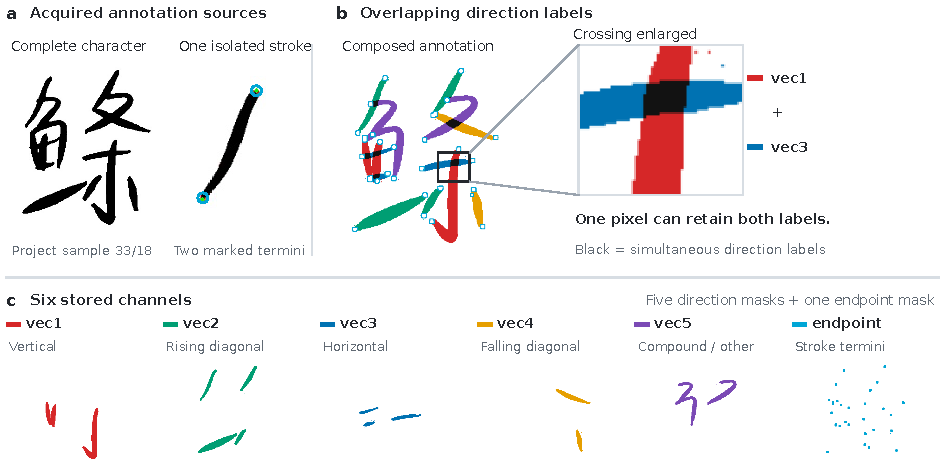
\includegraphics[width=\textwidth]{figures/revision/figure2_channel_definition.pdf}
  \caption{Six-channel overlapping annotation contract on one project
  sample (33/18). (a)~The complete character and one independently acquired
  stroke with two manually marked termini; cyan circles are display outlines.
  (b)~The composed annotation and an enlarged crossing of \(\mathrm{vec1}\)
  and \(\mathrm{vec3}\). Black pixels retain both direction labels rather
  than an exclusive class. (c)~The five direction channels and the endpoint
  channel, shown on a shared crop. The \(\mathrm{vec5}\) family includes
  compound, curved, and other non-cardinal strokes; the endpoint channel is
  the union of manually marked stroke termini, with dilation for display only.
  The software schema stores the channels as
  \((\mathrm{vec1},\ldots,\mathrm{vec5},\mathtt{keypoint})\); the last
  identifier is retained for backward compatibility and denotes this endpoint
  channel.}
  \label{fig:channel-definition}
\end{figure*}

The archive records preserve neither a trustworthy mapping from samples to
writers nor a standardized measure of contributor expertise, so the paper
makes no professional-calligrapher, different-writer, or writer-disjoint
claim.

\subsection{Quality control and split protocols}
\label{sec:data-qc}

Recovery of the acquisition archive yielded 894 sample directories across 43
character identities. Complete six-channel ground truth is available for 840
samples from identities 0--39; the 54 samples of identities 40--42 lack the
character-specific direction mapping and are excluded rather than
pseudo-labelled. A frozen semantic quality-control pass then identified 12
source-image/ground-truth mismatches and 59 non-canonical members of exact
image-and-mask duplicate groups. The two exclusion sets do not overlap,
leaving 769 unique QC-clean observations of 40 identities
(Fig.~\ref{fig:data-resources}a,b). All exclusion decisions were fixed before
the formal model comparison.

\begin{figure*}[!t]
  \centering
  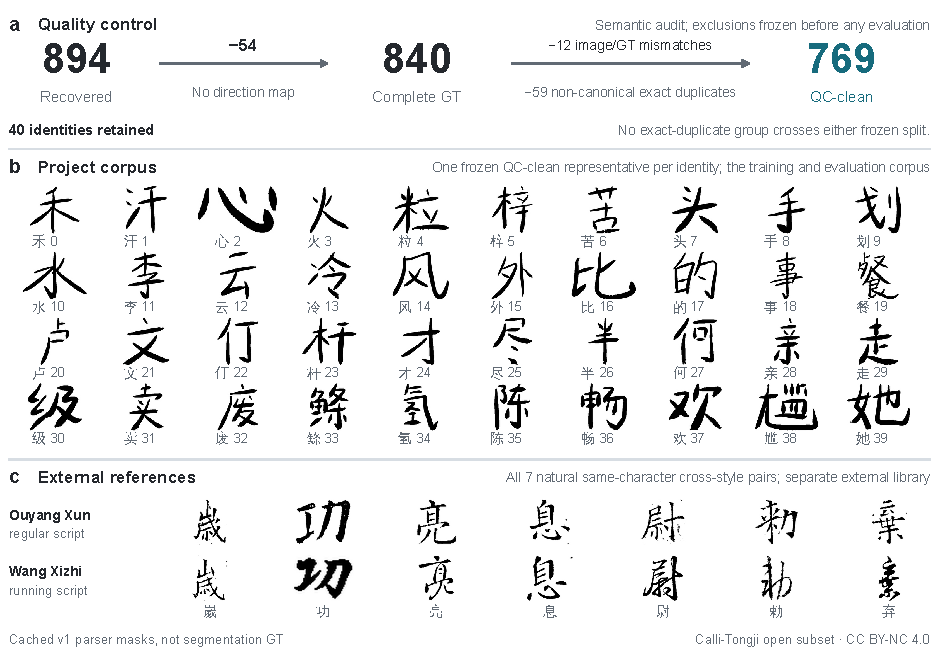
\includegraphics[width=\textwidth]{figures/revision/figure3_dataset_overview.pdf}
  \caption{Data resources and quality control. (a)~Recovery and exclusion
  audit: 54 of 894 recovered samples lack a direction mapping, leaving
  840 with complete six-channel ground truth. Removing 12 image/GT mismatches
  and 59 non-canonical exact duplicates yields 769 QC-clean observations of
  40 identities. No exact-duplicate group crosses either frozen split.
  (b)~One deterministic QC-clean observation per identity (IDs 0--39).
  (c)~All seven natural same-character cross-style pairs in the external
  library, represented by cached v1 parser masks, not segmentation ground
  truth. Source images: Calli-Tongji open subset \cite{yunmo_jixin_2025},
  CC~BY-NC~4.0.}
  \label{fig:data-resources}
\end{figure*}

Figure~\ref{fig:data-resources} shows the same audit graphically:
panel~(a) gives the exclusion flow and the retained identity count,
panel~(b) one deterministic QC-clean observation per retained identity so
that the character coverage of the corpus is visible at a glance, and
panel~(c) the seven natural cross-style pairs of the separate reference
library, whose cached masks are parser outputs rather than annotated ground
truth.

Two split protocols are used. The \emph{standard} assignment was frozen
before quality control by per-character sample index, with the same index
ranges in every identity, and contains 600/120/120 train/validation/test
samples before quality control and 530/119/120 after it; it measures
in-corpus generalization to new instances of seen identities. The
\emph{character-disjoint} assignment was frozen at the identity level before
any formal evaluation, with 28/6/6 disjoint identities and 588/126/126
samples before quality control and 539/114/116 after it; it measures
transfer to identities never seen in training. No exact-duplicate group
crosses either split.

\subsection{External reference library and derived cohorts}
\label{sec:data-references}

The reference-conditioned experiments use 200 approved images from the
publicly downloadable open subset of Calli-Tongji \cite{yunmo_jixin_2025}
(50 calligrapher--script categories with 100 samples each, released under
CC~BY-NC~4.0): the 100 images of the Ouyang Xun regular-script category and
the 100 images of the Wang Xizhi running-script category. Each
reference is parsed once by a frozen SegFormer-B2 checkpoint (version v1,
trained with the recipe of Sect.~\ref{sec:setup-parser} on the
pre-quality-control standard assignment and frozen before the formal
three-seed comparison), and the resulting six binary masks are cached with their provenance. These cached masks are model-derived reference
representations; they are never treated as segmentation ground truth and
never enter parser training.

Two cohorts are derived deterministically from the cached masks. The
\emph{perturbation cohort} applies the nuisance and structural edits of
Sect.~\ref{sec:setup-registration} to every reference, so that registration
and score behaviour can be studied without a second parser inference. The
\emph{cross-reference cohort} contains all seven natural
same-character cross-style pairs that the library supports
(Fig.~\ref{fig:data-resources}c) and 50 different-character negatives selected independently of any model score; the
library contains no same-style, different-instance reference pair. The perturbation cohort also serves as the diagnostic cohort of
Sect.~\ref{sec:setup-diagnostic}, where each known intervention is the
ground truth.

\subsection{Human-rating development cohort}
\label{sec:data-human}

Before any rating was collected, 150 natural same-character,
different-instance pairs were selected from the 769 QC-clean project samples,
three or four per identity, excluding mismatches, exact and suspected near
duplicates, and repeated instances. Pair roles, asset hashes, blinded
identifiers, and display order were frozen, and all automated scores and
source identifiers were hidden from the raters.

Three adult raters independently judged structural similarity on
a five-point ordinal scale, each rating the 150 canonical pairs plus 15
interspersed hidden repeats. The panel comprised two author-raters
with prior calligraphy study, one of whom holds a Level-9 calligraphy
certificate, and one non-author rater with master's-level training in Fine
Arts (Calligraphy). The panel is small, domain-qualified, and partly
author-involved; it is not an independent expert cohort. The main score
comparisons use the annotated masks of both instances, and the paired
direct-ink control uses thresholded source rasters. Neither includes parser
inference, so these comparisons assess score validity without parser error.
The ratings are the ASDS development data of
Sect.~\ref{sec:setup-human}, not an external test set.

\section{Method}
\label{sec:method}

\subsection{Overview and relation to prior formulations}

Let \(I_u\) be a learner image and \(I_r\) an approved reference image of
the same target character, one that passed the licence and quality review
of the reference library (Sect.~\ref{sec:data-references}); in deployment the system never scores images of different characters. The system parses both images into overlapping
structural masks, registers the reference to the learner with a restricted
global transform, and returns (i)~six masks per image, (ii)~a scalar
structural-agreement score, and (iii)~localized evidence
(Fig.~\ref{fig:pipeline}). The learner image is called the candidate in the
figures and \texttt{user} in the software contract; the terms denote the
same image. Three decisions distinguish this
formulation from the work of Sect.~\ref{sec:related}. Unlike Stroke-Seg
\cite{gong2024strokeseg}, which recovers individual strokes with a
character-specific composition prior supplied as input, the parser predicts
five direction families that may overlap plus a separate endpoint channel,
uses no per-character prior at inference, and feeds a reference-conditioned
comparison rather than a stroke inventory. The comparison is not a learned
pairwise similarity network \cite{chen2025siamhcc}; every score is a fixed,
decomposable function of aligned masks whose semantics can be audited.
Registration is a bounded similarity transform rather than a learned or
deformable warp \cite{jaderberg2015stn,zitova2003registration}
(Sect.~\ref{sec:alignment-method}).

\subsection{Overlapping six-channel parser}
\label{sec:parser}

For an RGB character image \(I\), a parser \(f_\theta\) predicts
\[
P=f_\theta(I)\in[0,1]^{H\times W\times 6},
\]
whose channels follow the annotation contract of
Sect.~\ref{sec:data-corpus}: five direction families and the endpoint
channel. Because a crossing pixel may carry several direction labels, each
channel is activated by an independent sigmoid rather than by a mutually
exclusive softmax; the five direction outputs may therefore overlap, exactly
as the composed ground truth does. For direction channel \(c\), the loss combines class-weighted
binary cross entropy (BCE) and soft Dice, averaged over the five channels,
\[
\mathcal{L}_{\mathrm{dir}}
=\frac{1}{5}\sum_{c=1}^{5}
\left(
\mathcal{L}_{\mathrm{BCE}}^{(c)}
+\mathcal{L}_{\mathrm{Dice}}^{(c)}
\right).
\]
The sparse endpoint target uses focal loss with \(\gamma=2\) and
\(\alpha=0.75\) plus Dice loss, and a boundary term derived from the masks is
weighted by \(0.2\):
\[
\mathcal{L}
=\mathcal{L}_{\mathrm{dir}}
+\mathcal{L}_{\mathrm{focal,end}}
+\mathcal{L}_{\mathrm{Dice,end}}
+0.2\,\mathcal{L}_{\mathrm{boundary}}.
\]
Binary masks are obtained from \(P\) with per-channel thresholds calibrated
on validation data only (Sect.~\ref{sec:setup-parser}).

\subsection{Reference cache and constrained registration}
\label{sec:alignment-method}

Let \(U\) and \(R\) denote the learner and cached reference binary stacks
(Sect.~\ref{sec:data-references}) and let
\[
M(X)=\bigvee_{c=1}^{5}X_c
\]
be the union of direction ink. For each candidate isotropic scale \(s\) and
rotation \(\phi\), the transformed reference is translated so that its
foreground centroid approaches the learner centroid. The production search
evaluates nine evenly spaced scales and seven evenly spaced rotations in
\[
s\in[0.8,1.2],\qquad \phi\in[-3^\circ,3^\circ],
\]
and selects the candidate maximizing the foreground intersection over union
(IoU) \(J\bigl(M(U),M(T_{s,\phi,t}(R))\bigr)\). Non-uniform scale, shear,
thin-plate splines, and deformable warping are disallowed. This bounded
search is a conservative compensation policy: it can absorb page placement
and modest global size or rotation differences while leaving local
proportion and stroke-region errors available for diagnosis; it implies no
invariance within the nominal range, and residual sensitivity is measured in
Sect.~\ref{sec:rq2}.

\subsection{Structural agreement scores}
\label{sec:scores}

Three scores are studied. Each is a fixed function of the aligned masks and
uses no character identity, writer identity, style identity, or human rating
at inference.

\medskip
\noindent\textbf{Frozen production score.}
After alignment, let \(D_c\) be Dice agreement in direction channel \(c\),
\(\overline{D}=\tfrac{1}{5}\sum_{c=1}^{5}D_c\), let \(J_{\mathrm{ink}}\) be
union-ink IoU, and let \(F_{\mathrm{end}}^{(3)}\) be endpoint-mask F1 with a
three-pixel tolerance. The deployed score is
\[
S_{\mathrm{prod}}
=100\left(
0.55\,\overline{D}
+0.25\,J_{\mathrm{ink}}
+0.20\,F_{\mathrm{end}}^{(3)}
\right).
\]
It was frozen before the controlled experiments and is never retuned in
this paper.

\medskip
\noindent\textbf{Coverage-aware score.}
The production Dice convention returns 1 for a channel that is empty in both
images, so a character that uses fewer direction families can receive credit
for structure that is absent. The coverage-aware score keeps the same
evidence families and weights but averages Dice only over direction channels
active in at least one image, and treats both-empty endpoint masks as
unavailable evidence with the remaining weights renormalized. It is reported alongside \(S_{\mathrm{prod}}\) as an audit variant and does
not replace it.

\medskip
\noindent\textbf{Aligned spatial-distribution similarity (ASDS).}
Pixel- and channel-overlap terms say little about how ink mass is organized
across the canvas. ASDS therefore compares three spatial distributions of
the union silhouette \(M(\cdot)\) after the same frozen registration. \emph{Polar occupancy} centres the foreground at
its ink centroid, divides radius by the 95th percentile of foreground radius
(clipped to \([0,1)\)), and assigns pixels to four radial and eight angular
bins, giving a normalized 32-bin histogram \(h_p\); by construction,
centroid and radius normalization make it insensitive to residual
translation and isotropic rescaling of the aligned silhouette, a property
not separately measured here. \emph{Grid occupancy} \(h_g\) counts normalized foreground over a
\(3\times3\) partition of the canvas and retains coarse location and
balance. \emph{Projection profiles} \(h_x\) and \(h_y\) are the normalized
column and row sums. For distributions \(p\) and \(q\) with \(m=(p+q)/2\), the
Jensen--Shannon divergence and the Jensen--Shannon similarity (JSS) are
\[
D_{\mathrm{JS}}(p,q)
=\tfrac{1}{2}D_{\mathrm{KL}}(p\Vert m)
+\tfrac{1}{2}D_{\mathrm{KL}}(q\Vert m),
\]
\[
\operatorname{JSS}(p,q)=1-\sqrt{D_{\mathrm{JS}}(p,q)},
\]
with base-2 logarithms, so that \(\operatorname{JSS}\in[0,1]\)
\cite{lin1991jensen}. With
\(s_p=\operatorname{JSS}(h_p(U),h_p(R))\),
\(s_g=\operatorname{JSS}(h_g(U),h_g(R))\), and
\(s_{\mathrm{proj}}\) the mean of the column and row similarities, the
frozen specification is
\[
S_{\asds}=100\bigl(
0.70\,s_p+0.15\,s_g+0.15\,s_{\mathrm{proj}}
\bigr).
\]
ASDS was developed after the ratings of Sect.~\ref{sec:data-human} were
available and its weights were selected on them
(Sect.~\ref{sec:setup-human}). Because it consumes only the union silhouette, it does not use the direction
semantics of the six-channel masks; whether those masks contribute anything
to this scalar beyond their silhouette is tested by the direct-ink control
(Sect.~\ref{sec:rq3}).

\subsection{Localized evidence and feedback}
\label{sec:evidence}

Alongside the scores, the system preserves the selected transform, the
pre-alignment centre distance and ink-area ratio, per-direction Dice, and
endpoint agreement. Difference masks between the aligned stacks are
summarized by direction channel, by type (reference ink missing from the
learner versus extra learner ink), and by a \(3\times3\) region set;
connected components are exposed as direction-classified regions, not as
recovered strokes or stroke order.
Deterministic rules rank centre, scale, endpoint, and local-direction
findings. An optional text model receives only this structured contract; it may
improve fluency but cannot change the score or add brushwork or stroke-order
claims the evidence does not contain.

\section{Experimental Setup}
\label{sec:setup}

This section states how each research question is tested; the cohorts
themselves are defined in Sect.~\ref{sec:data}.

\subsection{Parser training and evaluation (RQ1)}
\label{sec:setup-parser}

Three architectures are compared: a U-Net with 32 base channels, a ResNet-50
DeepLabV3+, and SegFormer-B2. U-Net has no external pretraining; all of its parameters are randomly
initialized. DeepLabV3+ loads the torchvision default ImageNet-1K weights for
its ResNet-50 encoder, while its atrous spatial pyramid pooling (ASPP)
module, low-level projection, decoder,
and six-channel output head are randomly initialized. SegFormer-B2 is
initialized from \texttt{nvidia/segformer-b2-finetuned-}\allowbreak
\texttt{ade-512-512}: the compatible Mix Transformer (MiT-B2) encoder and decode-head
parameters are loaded from the ADE20K-fine-tuned checkpoint, the incompatible
150-class classifier is replaced by a randomly initialized six-channel
classifier, and all layers are then fine-tuned. Each architecture is trained
with seeds 20260811, 314159, and 271828 on both split protocols, giving 18
formal runs.

Inputs are letterboxed to \(512\times512\) and normalized, and masks are
resized by nearest-neighbour interpolation. Batch size is 8 for U-Net and 4 for the two
larger models. Label-safe augmentation comprises translation up to 12
pixels, isotropic scale 0.9--1.1, brightness 0.85--1.15, contrast 0.9--1.1,
and Gaussian blur with probability 0.15. All models use AdamW with weight
decay 0.01, automatic mixed precision, gradient clipping at 1.0, three
warm-up epochs, cosine decay to \(10^{-6}\), at most 120 epochs, and early
stopping with patience 15. U-Net uses learning rate \(3\times10^{-4}\);
DeepLabV3+ uses encoder/decoder rates \(10^{-4}/10^{-3}\); SegFormer-B2 uses
\(3\times10^{-5}/3\times10^{-4}\). Positive BCE weights are estimated from at
most 200 training samples and capped at 100. Per-channel thresholds are
calibrated on the validation split only, and the test split is evaluated
once per run.

Direction quality is reported as five-direction Macro Dice and Macro IoU
between thresholded predictions and ground truth, and as Boundary F1, the F1
between the one-pixel morphological boundaries of prediction and ground
truth averaged over the five direction channels; endpoint quality is
reported as strict endpoint F1, the pixel-exact F1 on the endpoint channel,
unlike the three-pixel-tolerant term inside the production score. Test results are summarized as the mean and sample standard deviation
over the three seeds. The standard protocol measures in-corpus instance
generalization; the character-disjoint protocol measures transfer to unseen
characters.

\subsection{Registration and score-behaviour experiments (RQ2)}
\label{sec:setup-registration}

Controlled perturbations are applied directly to the 200 cached reference
masks. The nuisance family, for which a useful registration should show
little sensitivity, comprises translation, rotation, scale up, scale down,
and a compound transform. The structural family, for which the score should
decrease with severity, comprises terminal deletion, added direction
fragment, local fragment shift, direction dilation, direction erosion, and
endpoint shift. Each perturbation is applied at four severity levels, except
rotation and the compound transform, which use three, so a perturbation with
no invalid case contributes 800 rows from the 200 references. The affected channel and axis are selected by stable hashes, never by model
error or manual choice. A transformed case that risks canvas clipping is
marked invalid with a recorded reason and excluded from valid-score
summaries; its fraction is reported. For every perturbation we report valid
\(N\), mean drop with a 95\% reference-level bootstrap confidence
interval (CI), invalid
fraction, and adjacent-severity monotonicity, the fraction of adjacent
severity steps at which the score does not increase; median, standard
deviation,
percentiles, and severity correlations are given in Online Resource~1,
Table~S1.

The identical reference/perturbation/severity tuples are then scored under
three alignment policies: no alignment, the production constrained search of
Sect.~\ref{sec:alignment-method}, and a wider similarity search over the same grid with
\(s\in[0.6,1.4]\) and \(\phi\in[-12^\circ,12^\circ]\), fixed in the
frozen experiment contract before any result was computed.
Comparisons are paired by reference. Confidence intervals resample
references; Wilcoxon signed-rank tests \cite{wilcoxon1945} and rank-biserial
correlation (RBC) effect sizes use per-reference mean paired differences. Family-level
comparisons are the primary ablation; perturbation-level results are
descriptive and unadjusted (Online Resource~1, Table~S2).

Two semantic audits accompany the ablation. The inactive-channel audit
counts references with empty direction channels and recomputes the
coverage-aware score of Sect.~\ref{sec:scores} on every valid perturbation
row (Online Resource~1, Table~S3). The cross-reference test scores the seven
same-character cross-style pairs and the 50 different-character negatives
with \(S_{\mathrm{prod}}\) and summarizes their separation with Cliff's
\(\delta\) \cite{cliff1993dominance}; self-pairs are prohibited.

\subsection{Human-association study and ASDS development (RQ3)}
\label{sec:setup-human}

Each score is compared with the three-rater mean on the 150 canonical pairs
by Spearman correlation, with 95\% intervals from 10,000 bootstrap resamples
clustered by target character \cite{efron1993bootstrap}. Two-sided \(p\) values for
\(\rho=0\) are reported for the two frozen scores. Inter-rater
reliability uses two-way random-effects, absolute-agreement intraclass
correlation coefficients ICC(2,1) and ICC(2,\(k\))
\cite{mcgraw1996icc,koo2016icc}. Hidden repeats are excluded from
correlation and ICC and are used only for exact agreement, agreement within
one point, mean absolute difference (MAD), and quadratic weighted kappa
(QWK).

\medskip
\noindent\textbf{Post-rating ASDS development.}
The original ratings are the ASDS development set. Three fixed distribution
families (polar, grid, projection) are considered, and a coarse non-negative
simplex search evaluates component weights against the ratings. The
search-selected polar weight is retained, and the remaining weight is split
equally between grid and projection to reduce sample-specific tuning; the full candidate search is reported in Online Resource~1, Note~S5. Five-fold
internal validation groups pairs by character identity and selects the
weights of each fold on the other characters only, giving a
character-grouped out-of-fold estimate. Character-cluster bootstrap intervals are reported for the frozen score,
the out-of-fold predictions, the components, and paired differences from
the production and coverage-aware scores; these comparisons are exploratory
and not multiplicity-adjusted.

\medskip
\noindent\textbf{Paired direct-ink control.}
To test whether the ASDS scalar itself requires six-channel masks, ASDS is
recomputed on the same 150 pairs with foreground taken directly from the
original rasters instead of from the union of the annotated direction
masks: grayscale pixels with intensity below 240, the threshold
already frozen for dataset quality control, define ink, with no learned
preprocessing. Direct-ink masks pass through the same constrained
registration and frozen formula; nothing is selected against the ratings for
this comparison. We report the Spearman association of the annotated-mask-union variant
(the ``parsed union'' of the frozen artifact) and the direct-ink variant with the
ratings, their
paired difference, and their mutual rank association, with 10,000 paired
resamples clustered by character. Because the control reuses the development
pairs, it measures implementation dependence within the same retrospective
cohort, not external validity.

\subsection{Diagnostic evaluation (RQ4)}
\label{sec:setup-diagnostic}

The diagnostic cohort applies every severity level of the 11 perturbations
to the 200 references; the known perturbation of each case supplies
deterministic ground truth for the direction channel, the missing/extra
type, and the affected \(3\times3\) cells. The required finding is the centre-offset
finding for translation, the ink-scale finding for scale changes, a local
direction finding for the five direction edits, and the endpoint-relation
finding for endpoint shifts; rotation and compound cases have no required
finding. We report required Recall@3, the fraction of cases whose required
finding appears among the top three returned findings, and exact grid
localization, which counts a case as
correct only when the returned cell equals the truth cell set and is scored
on the cases whose perturbation edits a direction channel. Each exact-localization failure is assigned one primary cause in the fixed
order local finding absent from the top three, wrong direction channel,
wrong missing/extra type, multi-cell or grid-boundary truth, and alignment
residual shift; direction and type errors are characterized only through
this classification, and language-model realization is disabled.

\section{Results and Discussion by Research Question}
\label{sec:results}

Results are organized by research question. All reported values come from
frozen experiment artifacts; Online Resource~1, Note~S6, lists the integrity
hashes of those included in the code release.

\subsection{RQ1 (representation and generalization)}
\label{sec:rq1}

RQ1 is answered by the 18 formal runs of Sect.~\ref{sec:setup-parser} on
the standard and character-disjoint splits (Table~\ref{tab:segmentation})
and by the qualitative comparison of
Fig.~\ref{fig:segmentation-qualitative}.

\begin{table*}[t]
\centering
\caption{Segmentation results over three fixed random seeds on the QC-clean
standard split and the character-disjoint split (train, validation, and test
identities disjoint). Values are mean \(\pm\) sample standard deviation;
Endpoint F1 is the strict pixel-level score; bold marks the best value in
each column within a split.}
\label{tab:segmentation}
\footnotesize
\begin{tabular}{llcccc}
\toprule
Split & Model & Macro Dice & Macro IoU & Endpoint F1 & Boundary F1 \\
\midrule
\multirow{3}{*}{Standard}
  & U-Net
  & \(0.9196 \pm 0.0018\)
  & \(0.8515 \pm 0.0030\)
  & \(\mathbf{0.7562 \pm 0.0038}\)
  & \(0.8009 \pm 0.0023\) \\
  & DeepLabV3+
  & \(\mathbf{0.9630 \pm 0.0006}\)
  & \(\mathbf{0.9287 \pm 0.0012}\)
  & \(0.7218 \pm 0.0012\)
  & \(\mathbf{0.8443 \pm 0.0028}\) \\
  & SegFormer-B2
  & \(0.9581 \pm 0.0031\)
  & \(0.9196 \pm 0.0057\)
  & \(0.7139 \pm 0.0046\)
  & \(0.8259 \pm 0.0088\) \\
\midrule
\multirow{3}{*}{Character-disjoint}
  & U-Net
  & \(0.8260 \pm 0.0161\)
  & \(0.7120 \pm 0.0225\)
  & \(\mathbf{0.6972 \pm 0.0045}\)
  & \(0.6430 \pm 0.0136\) \\
  & DeepLabV3+
  & \(0.8664 \pm 0.0094\)
  & \(0.7663 \pm 0.0146\)
  & \(0.6755 \pm 0.0031\)
  & \(0.6728 \pm 0.0138\) \\
  & SegFormer-B2
  & \(\mathbf{0.8866 \pm 0.0008}\)
  & \(\mathbf{0.7977 \pm 0.0013}\)
  & \(0.6604 \pm 0.0033\)
  & \(\mathbf{0.6851 \pm 0.0046}\) \\
\bottomrule
\end{tabular}
\end{table*}


On the standard split, DeepLabV3+ obtains the highest direction Macro Dice
(\(0.9630\pm0.0006\)), Macro IoU (\(0.9287\pm0.0012\)), and Boundary F1
(\(0.8443\pm0.0028\)). U-Net is weaker on direction and boundary
metrics yet gives the best strict endpoint F1 (\(0.7562\pm0.0038\)). Dense
direction segmentation and sparse endpoint localization therefore favour
different model configurations.



All models degrade when character identities are held out
(Table~\ref{tab:segmentation}, bottom). SegFormer-B2
gives the strongest character-disjoint direction result: Macro Dice
\(0.8866\pm0.0008\), Macro IoU \(0.7977\pm0.0013\), and Boundary F1
\(0.6851\pm0.0046\). Its Macro-Dice decrease from the standard split is 7.150
percentage points, versus 9.664 for DeepLabV3+ and 9.360 for U-Net.
DeepLabV3+ remains second for direction overlap, and U-Net retains the
highest strict endpoint F1 (\(0.6972\pm0.0045\)). Near-saturated in-corpus
overlap thus does not imply transfer to unseen character structures, and the
best-performing configuration on held-out identities differs from the
standard-split leader. These comparisons include the initialization and
training choices of Sect.~\ref{sec:setup-parser}, rather than isolating
architecture alone.

\begin{figure*}[!t]
  \centering
  
\includegraphics[width=\textwidth]{figures/redrawn/figure4_segmentation_qualitative.pdf}
  \caption{Frozen qualitative comparison for seed 20260811 on a
  multi-channel crossing, an endpoint-rich case, and a held-out character
  (samples are identified as identity/sample index).
  The first two rows use standard-split models and the third uses
  character-disjoint models. Call-outs are identical across columns: the
  circle in (a) marks a crossing where every model emits two labels, the box
  in (b) two short strokes whose endpoints every model keeps, and the boxes
  in (c) black smears and swapped labels on the held-out identity. Values
  under (c) are the dataset-level character-disjoint Macro Dice of
  Table~\ref{tab:segmentation}. Colours follow
  Fig.~\ref{fig:channel-definition}; thresholds are validation-calibrated.}
  \label{fig:segmentation-qualitative}
\end{figure*}

Figure~\ref{fig:segmentation-qualitative} makes the output contract
visible: at the crossing in the first row every model emits overlapping
labels rather than choosing one family, and the third row shows the errors
characteristic of an identity absent from training.

\medskip
\noindent\textbf{Answer to RQ1.}
The best model configuration depends on the target and split:
DeepLabV3+ leads in-corpus direction parsing, SegFormer-B2 unseen-character
direction parsing, and U-Net strict endpoint localization. Holding out
identities costs 7.150--9.664 Macro-Dice points. Crossing agreement is shown
qualitatively, not measured separately; character-disjoint testing measures
transfer within one acquisition source, not to unseen writers.

\subsection{RQ2 (registration and score behaviour)}
\label{sec:rq2}

RQ2 is answered by the controlled-perturbation summary
(Table~\ref{tab:controlled}), the paired alignment ablation
(Table~\ref{tab:alignment}, Fig.~\ref{fig:alignment-ablation}), the inactive-channel audit, and the cross-reference test (Online Resource~1,
Table~S4) described in Sect.~\ref{sec:setup-registration}.

\begin{table*}[t]
\caption{Controlled perturbation summary. Nuisance rows report absolute score
drop; structural rows report signed drop from identity. Full distribution and
severity statistics are in Supplementary Table S1.}
\label{tab:controlled}
\centering
\scriptsize
\begin{tabular}{lrrrrr}
\toprule
Perturbation & Valid \(N\) & Mean drop & 95\% CI & Invalid fraction & Monotonic \\
\midrule
Translation & 800 & 0.000 & [0.000, 0.000] & 0.000 & 1.000 \\
Rotation & 520 & 5.395 & [5.079, 5.747] & 0.133 & 0.647 \\
Scale up & 408 & 13.653 & [12.964, 14.420] & 0.490 & 0.271 \\
Scale down & 800 & 16.356 & [15.670, 17.074] & 0.000 & 0.500 \\
Compound allowed transform & 276 & 8.143 & [7.621, 8.717] & 0.540 & 0.466 \\
Terminal deletion & 800 & 19.757 & [17.387, 22.087] & 0.000 & 0.992 \\
Added direction fragment & 800 & 11.398 & [9.934, 12.929] & 0.000 & 0.987 \\
Local fragment shift & 800 & 4.310 & [3.886, 4.772] & 0.000 & 0.985 \\
Direction dilation & 800 & 24.034 & [22.180, 25.955] & 0.000 & 1.000 \\
Direction erosion & 800 & 22.225 & [20.269, 24.344] & 0.000 & 0.997 \\
Keypoint shift & 800 & 7.468 & [7.294, 7.641] & 0.000 & 1.000 \\
\bottomrule
\end{tabular}
\end{table*}


Under the production registration, translation is recovered exactly in all
800 valid cases, whereas residual sensitivity remains for the other
transforms: mean penalties are 5.395 points for rotation, 13.653 for scale
up, and 16.356 for scale down. Scale up and the compound transform have
invalid fractions of 49.0\% and 54.0\% because of clipping risk, so their
summaries hold only for clipping-safe references and establish no invariance
across the library. Among structural perturbations, direction dilation
and erosion produce the largest penalties, followed by terminal deletion and
added fragments; local fragment shifts and endpoint shifts are weaker but
monotonic in severity.

\begin{table*}[t]
\caption{Paired alignment comparison. Positive benefit differences favour the
current constrained alignment and are computed from unrounded means. Ours is
the production constrained search of Sect.~\ref{sec:alignment-method};
Comparator is no alignment (none) or the wider search (wide); values are
mean score drops; RBC is the rank-biserial correlation. Wilcoxon tests use
per-reference mean paired differences.}
\label{tab:alignment}
\centering
\footnotesize
\begin{tabular}{llrrrrrrr}
\toprule
Comparison & Family & Refs & Ours & Comparator & Benefit 95\% CI & $p$ & RBC \\
\midrule
Ours--none & nuisance & 200 & 8.455 & 38.573 & [29.506, 30.727] & \(<0.001\) & 1.000 \\
Ours--none & structural & 200 & 14.865 & 3.677 & [10.094, 12.322] & \(<0.001\) & 1.000 \\
Ours--wide & nuisance & 200 & 8.455 & 11.351 & [2.757, 3.034] & \(<0.001\) & 1.000 \\
Ours--wide & structural & 200 & 14.865 & 15.149 & [-0.355, -0.213] & \(<0.001\) & -0.683 \\
\bottomrule
\end{tabular}
\end{table*}


The paired comparison isolates what registration buys. Relative to no
alignment, the constrained search reduces the nuisance penalty by 30.118
points (reference-bootstrap 95\% CI 29.506--30.727) and increases the penalty
for the tested structural interventions by 11.189 points (10.094--12.322);
both per-reference signed-rank comparisons are nonzero with rank-biserial
effect size 1.0. Without alignment the same structural edits cost only 3.677 points on
average against 14.865 under registration
(Fig.~\ref{fig:alignment-ablation}c), so the constrained search does not
suppress structural penalties; part of the increase may reflect the centroid-derived translation re-fitting
the whole reference after a local edit. The wider, coarser search incurs a 2.896-point higher nuisance
penalty (2.757--3.034) while preserving only 0.284
additional points of structural penalty. This tested search configuration
does not improve the measured trade-off (perturbation-level results in
Online Resource~1, Table~S2).

\begin{figure*}[!t]
  \centering
  
\includegraphics[width=\textwidth]{figures/redrawn/figure5_alignment_ablation.pdf}
  \caption{Alignment ablation on deterministic translation, scale-down, and
  terminal-deletion cases of one reference. Columns compare no alignment, the
  production range, and the wider search; dark grey, blue (dashed outline),
  and red (solid outline) denote overlap, missing reference ink, and extra
  candidate ink. The right-hand column plots the score drop (100 minus
  score) of each condition on one 0--100 axis, with an arrow from no
  alignment to the production range; rows (a)--(b) are nuisance
  perturbations whose drop should vanish, row (c) a structural edit whose
  drop should remain. Registration removes the translation penalty in row (a), reduces but does not eliminate
  the scale penalty in row (b), and retains the structural penalty in
  row (c). Source reference: Calli-Tongji open subset
  \cite{yunmo_jixin_2025}, CC~BY-NC~4.0.}
  \label{fig:alignment-ablation}
\end{figure*}


Forty-one
of the 200 references contain inactive direction channels (36 with one and
five with two; Online Resource~1, Table~S3). Both-empty agreement affects 1,252 of
the 7,604 valid perturbation rows, and averaging over active channels changes
\(S_{\mathrm{prod}}\) by \(-0.289\) points on average and by at most
\(-15.402\): macro overlap can reward absent structure, which motivates the
coverage-aware score tested in RQ3.



In the cross-reference test (Online Resource~1, Table~S4), the seven
same-character cross-style pairs score 20.239 on average (95\% CI 15.639--25.069) against 9.741
(8.584--10.970) for the 50 different-character negatives, with Cliff's
\(\delta=0.84\). The score carries same-character signal across styles, but the small
positive set and the missing same-style condition preclude a broader claim.

\medskip
\noindent\textbf{Answer to RQ2.}
Constrained registration reduces nuisance penalties while retaining
sensitivity to structural edits. The tested wider, coarser search does not
improve this trade-off. Residual rotation and scale penalties and clipping
exclusions bound the claim. The cross-reference test shows same-character
signal, while the inactive-channel audit exposes credit for absent
structure, motivating explicit coverage semantics.

\subsection{RQ3 (human validity)}
\label{sec:rq3}

RQ3 is answered on the 150-pair human-rating cohort of
Sect.~\ref{sec:data-human} with the statistics of
Sect.~\ref{sec:setup-human}: association of the frozen scores
(Table~\ref{tab:human-validation}), rater reliability
(Table~\ref{tab:rater-reliability}), ASDS development
(Table~\ref{tab:spatial-score-development}), and the direct-ink control
(Table~\ref{tab:direct-ink-asds}, Fig.~\ref{fig:asds-direct-ink}).

\begin{table}[t]
\caption{Association between the structural scores and the mean rating of
three blinded human raters across 150 canonical pairs. Confidence intervals
use 10,000 bootstrap resamples clustered by character.}
\label{tab:human-validation}
\centering
\scriptsize
\setlength{\tabcolsep}{3pt}
\begin{tabular}{lccc}
\toprule
Score & \(\rho\) & 95\% CI & \(p\) \\
\midrule
Production & 0.297 & [0.148, 0.441] & \(2.28\times10^{-4}\) \\
Coverage-aware & 0.429 & [0.313, 0.535] & \(4.32\times10^{-8}\) \\
\bottomrule
\end{tabular}
\end{table}

\begin{table}[t]
\caption{Calligraphy-domain-rater reliability. ICC uses only the 150 canonical
presentations. Repeat statistics use the 15 hidden repeats per rater: Exact
and Within \(\pm1\) are agreement fractions between canonical and repeat
ratings, MAD the mean absolute difference, and QWK the quadratic weighted
kappa; E01--E03 are blinded rater codes and POOLED aggregates all repeats.}
\label{tab:rater-reliability}
\centering
\small
\begin{tabular}{lrrrr}
\toprule
Rater & Exact & Within $\pm 1$ & MAD & QWK \\
\midrule
E01 & 0.600 & 1.000 & 0.400 & 0.559 \\
E02 & 0.467 & 1.000 & 0.533 & 0.721 \\
E03 & 0.400 & 0.800 & 0.800 & 0.591 \\
POOLED & 0.489 & 0.933 & 0.578 & 0.634 \\
\bottomrule
\end{tabular}
\vspace{2pt}
\begin{minipage}{0.96\columnwidth}\footnotesize
Canonical ICC(2,1)=0.448 and
ICC(2,$k$)=0.709 for
150 pairs and 3 raters.
\end{minipage}
\end{table}


The frozen production score correlates modestly with the three-rater mean
(\(\rho=0.297\), character-cluster 95\% CI 0.148--0.441), and the
coverage-aware score is stronger (\(\rho=0.429\), 0.313--0.535); their
paired difference is 0.132 (0.062--0.197). Single-rater reliability is below the 0.50 threshold that Koo and Li
\cite{koo2016icc} label moderate (ICC(2,1) 0.448), whereas the three-rater
mean is moderate (ICC(2,\(k\)) 0.709); hidden repeats yield
48.9\% exact agreement, 93.3\% agreement within one point, MAD 0.578, and
pooled QWK 0.634.

\begin{table}[t]
\caption{Development-stage ASDS association with mean human rating
(character-cluster bootstrap 95\% CI).}
\label{tab:spatial-score-development}
\centering
\scriptsize
\setlength{\tabcolsep}{3pt}
\begin{tabular}{@{}lcc@{}}
\toprule
Score or component & Spearman \(\rho\) & 95\% CI \\
\midrule
Grid only & 0.447 & [0.303, 0.572] \\
Projection only & 0.445 & [0.316, 0.564] \\
Polar only & 0.547 & [0.443, 0.645] \\
ASDS (frozen) & 0.556 & [0.454, 0.651] \\
ASDS (grouped OOF) & 0.540 & [0.432, 0.639] \\
\bottomrule
\end{tabular}
\end{table}


ASDS reaches \(\rho=0.556\) (0.454--0.651), and character-grouped
out-of-fold weight selection retains \(\rho=0.540\) (0.432--0.639). The
paired intervals for ASDS minus the production and coverage-aware scores are
0.110--0.410 and 0.017--0.239; the out-of-fold difference from the
coverage-aware score is less certain (\(-0.003\)--0.224). The polar component
is the strongest single term (\(\rho=0.547\)); grid and projection reach
0.447 and 0.445. Because the same ratings informed feature design, \(\rho=0.556\) is a
retrospective development result, and \(\rho=0.540\) is a
character-grouped internal-validation estimate that removes
weight-selection optimism only: the feature families were also chosen after
the ratings, so neither value is an external or prospective confirmation.

\begin{table}[t]
\caption{Direct-ink ablation of the frozen ASDS specification on the same 150
development pairs.}
\label{tab:direct-ink-asds}
\centering
\begin{tabular}{@{}lcc@{}}
\toprule
ASDS input & Spearman $\rho$ & 95\% CI \\
\midrule
Annotated-mask union & 0.556 & [0.454, 0.651] \\
Direct ink & 0.556 & [0.454, 0.649] \\
\midrule
$\Delta\rho$ (annotated--direct) & 0.000 & [-0.010, 0.010] \\
\bottomrule
\end{tabular}
\parbox{0.86\columnwidth}{\footnotesize\raggedright
Direct ink: grayscale intensity $<240$ (frozen QC threshold,
Sect.~\ref{sec:setup-human}); same registration, features, and weights for
both variants.}
\end{table}


The direct-ink control tests whether an annotated-mask union improves ASDS
association over thresholded source ink. Annotated-mask-union and direct-ink ASDS reach
\(\rho=0.55623\) and \(0.55583\);
their difference is \(\Delta\rho=0.00040\) (95\% CI
\(-0.01011\)--\(0.01030\); Table~\ref{tab:direct-ink-asds} rounds to
three decimals), and the two score vectors have rank association 0.9973
(Fig.~\ref{fig:asds-direct-ink}). On these clean direct-digital development pairs, thresholded ink and the
annotated-mask union yield closely matched human associations and score
rankings. This result supports the silhouette interpretation of ASDS, but
does not establish formal equivalence or transfer to degraded input.

\begin{figure*}[p]
  \centering
  
\includegraphics[width=\textwidth]{figures/revision/figure6_asds_direct_ink.pdf}
  \caption{ASDS mechanism and direct-ink control. (a)--(b)~A natural pair
  and its aligned silhouettes. (c)--(d)~Absolute polar (four radial by eight
  angular bins) and \(3\times3\) occupancy differences, each normalized
  to its own maximum; intensities are not comparable between maps.
  (e)~Projection profiles: rows solid, columns dashed; candidate red,
  reference blue. (f)~Frozen formula and example score. (g)~All 150 pairs
  from 40 identities. Annotated-mask union uses five manual direction masks,
  not parser predictions. Brackets are character-cluster bootstrap 95\% CIs;
  \(\Delta\rho\) is annotated-mask-union minus direct-ink association.
  Filled points identify the example; the right-hand dashed line is the
  identity. Observed associations and rankings are closely matched.}
  \label{fig:asds-direct-ink}
\end{figure*}

\medskip
\noindent\textbf{Answer to RQ3.}
ASDS has the strongest observed human association, but its internally
validated advantage over the coverage-aware score remains unresolved
(paired 95\% CI \(-0.003\)--0.224). Its silhouette formulation and the
direct-ink control separate scalar agreement from the parser's role in
direction and endpoint evidence. RQ1 evaluates parser accuracy; RQ4 tests
the downstream diagnostic mechanism under controlled mask interventions.
Human validity remains limited to structural agreement on one retrospective
cohort with three raters, two of them authors.

\subsection{RQ4 (localized diagnosis)}
\label{sec:rq4}

RQ4 is answered on the diagnostic cohort with the metrics of
Sect.~\ref{sec:setup-diagnostic} (Table~\ref{tab:feedback-failures},
Fig.~\ref{fig:diagnostic-cases}).

\begin{table}[t]
\caption{Primary taxonomy of exact-region diagnostic failures.}
\label{tab:feedback-failures}
\centering
\small
\begin{tabular}{lrr}
\toprule
Failure type & Count & Fraction \\
\midrule
multi\_region\_or\_grid\_boundary\_truth & 1922 & 0.539 \\
wrong\_direction\_channel & 876 & 0.246 \\
local\_finding\_absent\_from\_top3 & 718 & 0.201 \\
wrong\_missing\_extra\_type & 38 & 0.011 \\
alignment\_residual\_region\_shift & 11 & 0.003 \\
\bottomrule
\end{tabular}
\end{table}


Required Recall@3 is 0.701, whereas exact grid localization is 0.109. Under the fixed-order taxonomy, 53.9\% of exact-region failures are assigned
to multi-cell or grid-boundary truth, 24.6\% to wrong direction attribution,
and 20.1\% to a local finding absent from the top three. Figure~\ref{fig:diagnostic-cases} shows one exact
success and one audited failure of the first kind: the returned cell
overlaps the multi-cell change, and the frozen metric still records a
failure. The largest assigned category therefore reflects a mismatch between
spatial extent and the exact-cell metric, followed by direction attribution.
These categories concern structured evidence rather than wording.

\begin{figure*}[p]
  \centering
  
\includegraphics[width=\textwidth]{figures/redrawn/figure7_diagnostic_cases.pdf}
  \caption{Frozen diagnostic evidence: (a)~an exact-localization success
  and (b)~multi-cell truth classified as failure by the exact-one-cell metric.
  Findings report type~$|$ direction~$|$ missing/extra~$|$ cell; rXcY indexes
  the \(3\times3\) grid and \texttt{user} denotes the candidate.
  Dark grey is overlap, blue (dashed) missing reference ink, and red (solid)
  extra candidate ink. Solid and dashed black frames mark truth and predicted
  cells, respectively. Cards state the findings, truth, and audit verdict.
  The bottom strip summarizes Table~\ref{tab:feedback-failures} over
  3,565 exact-region failures; case (b) is in the largest assigned category.}
  \label{fig:diagnostic-cases}
\end{figure*}

\medskip
\noindent\textbf{Answer to RQ4.}
The evidence layer usually surfaces the required finding but does not
reliably assign it to one \(3\times3\) cell. Multi-cell truth and direction
attribution dominate the assigned failures. Wrong missing/extra type is the
primary category in 1.1\%, a lower bound under the fixed-order taxonomy.
These controlled interventions evaluate the diagnostic mechanism, not
teacher agreement or pedagogical usefulness.

\section{General Discussion and Limitations}
\label{sec:discussion}

\subsection{Implications for structural assessment}

The four research questions jointly define how structural differences are
represented, compensated, scored, and localized. Low-resource parsing must
be evaluated on the generalization axis relevant to the application,
because the best in-corpus parser did not transfer best to unseen
characters. These rankings describe the tested training protocols,
including their different initialization schemes. Overlapping labels retain
crossing evidence that a mutually exclusive pixel partition cannot express
(Fig.~\ref{fig:segmentation-qualitative}).

Registration shapes the measurement because the transform family
determines which discrepancies remain visible. The bounded search reduces
global nuisance penalties while retaining penalties for structural edits.
The increase in structural penalties can partly reflect centroid-based
refitting after a local edit; it does not independently establish better
measurement fidelity. The tested wider search also uses coarser sampling,
so its comparison does not isolate transform range. Residual sensitivity
prevents a claim of complete invariance under either search.

Scalar agreement and localized diagnostics require different evidence.
ASDS depends on the union silhouette, so permuting direction labels leaves
it unchanged. Such a change can alter directional comparisons and
localized attributions while leaving the separate endpoint mask unchanged.
The direct-ink control supports thresholded ink as an input for scalar
silhouette comparison in this cohort. Within this framework, the parser
supplies direction-specific and endpoint evidence unavailable from the
silhouette alone.

The frozen ASDS specification now requires evaluation without modification
on new writers, characters, and raters. Diagnostic localization also
requires region-overlap or pixel-overlap metrics that credit multi-cell
truth.

\subsection{Limitations}

The segmentation corpus contains 40 labelled character identities from one
recovered acquisition source. Character-disjoint evaluation does not
establish writer-disjoint generalization (Sect.~\ref{sec:data-corpus}), and
collection-specific regularities may survive semantic quality control.

Controlled perturbations operate on cached reference masks predicted by
the v1 checkpoint, which predates semantic quality control and the formal
comparison. Systematic parsing errors in those masks can propagate into
RQ2 and RQ4 statistics. Perturbed masks are compared directly without
rerunning the parser, so this benchmark does not measure end-to-end
performance on perturbed images. Scale-up and compound summaries are
conditional on clipping-safe references because their invalid fractions are
high. The external library supports only seven same-character cross-style
pairs, limiting conclusions about discrimination across styles.

The human cohort contains 150 pairs rated by three domain-qualified raters,
two of whom are authors. Single-rater reliability is poor, while reliability
of the three-rater mean is moderate. The primary score comparison uses
annotated masks, so it excludes deployment parser error; the direct-ink
control bypasses parsing. ASDS feature design followed inspection of the
ratings, making its association retrospective and its character-grouped
validation internal. The direct-ink control reuses this cohort and provides
no independent confirmation.

The contribution of registration to ASDS was not isolated. Its polar term
is centroid- and scale-normalized, so part of the observed association may
persist without alignment. Agreement at multi-label crossing pixels is not
measured separately, and diagnostic ground truth comes from engineered
interventions rather than teacher judgments. The supported modality remains
clean direct digital writing; robustness to camera capture has not been
evaluated (Sect.~\ref{sec:introduction}).

\section{Conclusion}
\label{sec:conclusion}

We presented an auditable framework for assessing a handwritten Chinese
character against a same-character reference under limited labelled data.
Overlapping parsing, constrained registration, and human-audited comparison
provide a shared basis for scalar agreement and localized evidence.

For RQ1, three parsers learn overlapping direction masks and a separate
endpoint mask from a 769-sample quality-controlled corpus. DeepLabV3+ leads
standard-split direction parsing, SegFormer-B2 leads character-disjoint
direction parsing, and U-Net leads strict endpoint localization. For RQ2,
constrained similarity registration reduces nuisance penalties by 30.118
points relative to no alignment while increasing structural penalties by
11.189 points. The tested wider, coarser search does not improve this
trade-off, and the reported benefit remains conditional on clipping-safe
references.

For RQ3, blinded ratings from three domain-qualified raters, including two
authors, associate most strongly with ASDS, followed by the coverage-aware
and frozen production scores. ASDS reaches \(\rho=0.556\) in retrospective
development and \(\rho=0.540\) under character-grouped internal validation.
Its internally validated advantage over the coverage-aware score remains
unresolved. Direct-ink and annotated-mask-union ASDS show nearly identical
association in this cohort. The parser supplies direction, overlap,
endpoint, and localized evidence beyond this scalar comparison. For RQ4,
controlled mask interventions show that the evidence layer usually surfaces
the required finding but does not reliably localize it to one cell.
Multi-cell or grid-boundary truth is the largest assigned failure category
(53.9\%) under the fixed-order taxonomy and exact-one-cell metric.

Together, these results support inspectable, reference-conditioned
structural assessment of clean direct-digital writing, with structured
evidence established before language generation. Independent human
validation and improved localization assessment remain necessary before
broader claims about aesthetic or pedagogical usefulness.


\backmatter

\section*{Acknowledgements}
The authors thank Chengcheng Wan for project supervision.

\section*{Statements and Declarations}

\bmhead{Funding}
This work was conducted within the East China Normal University Undergraduate
Innovation Training Incubation Project (Entrepreneurship Training category),
``OneStroke: A Vision-Model-Based Intelligent Feedback System for Chinese
Calligraphy''. No external funding channel is recorded, and no grant number
was available at the time of writing.

\bmhead{Competing Interests}
The authors declare no competing interests.

\bmhead{Ethics Approval}
Not applicable. The study analysed images of handwritten characters and
perceptual similarity ratings; it involved no clinical, medical, or
behavioural intervention on human subjects. The handwriting corpus was
commissioned by the project without recording writer identities, and the
structural-similarity ratings were provided by two of the authors and one
collaborating calligraphy specialist as part of the study design, stored under
evaluator codes, with no sensitive personal information collected.

\bmhead{Informed Consent}
Not applicable. No identifiable personal data of writers or raters are
reported; the three raters took part in the rating study voluntarily as
contributors to the project and were informed that the task assessed
character structure similarity, not their own ability.

\bmhead{Data Availability}
The frozen data contracts and result tables that support the reported values
are in the code repository named under Code Availability: the quality-control
audit and exclusion contract and both split assignments
(\path{artifacts/data_qc}, \path{artifacts/data_audit},
\path{artifacts/paper_ijdar/character_disjoint}); the per-seed
segmentation results and checkpoint manifest
(\path{artifacts/paper_ijdar/task1}); the ASDS development features,
character-grouped folds, frozen specification, and report
(\path{artifacts/paper_ijdar/spatial_score_development}); the 150-pair
direct-ink ASDS table (\path{artifacts/paper_ijdar/direct_ink_asds});
the reference-library manifest with per-image source paths and SHA-256
digests (\path{references/calli_tongji_beta_manifest.csv}); and the
figure provenance manifest. Online Resource~1, Note~S6, lists the digests of
every frozen artifact. The external reference images are the Ouyang Xun
regular-script and Wang Xizhi running-script categories (100 images each) of
the Calli-Tongji open subset \cite{yunmo_jixin_2025}, publicly downloadable
from ModelScope under CC~BY-NC~4.0 at
\url{https://www.modelscope.cn/datasets/CalliTongji/Calli-Tongji_A_Dataset_of_Historical_Calligraphy_Styles};
they are reproduced in Figs.~\ref{fig:pipeline}, \ref{fig:data-resources},
and~\ref{fig:alignment-ablation} with attribution and are not redistributed.
The project-collected handwriting images and six-channel masks, the
controlled-perturbation, alignment-ablation, inactive-channel, and
cross-reference result files, and the blinded 150-pair rating files
(evaluator codes only) are available from the corresponding author on
reasonable request for non-commercial research use.

\bmhead{Code Availability}
Source code, frozen experiment contracts, analysis scripts, and
non-restricted reproducibility artifacts are maintained at
\url{https://github.com/LiuXiaofan-0321/OneStroke2026}; an identity-free
archival copy will be supplied if anonymous review is required.

\bmhead{Author Contributions}
X.L.: Conceptualization, methodology, software, formal analysis,
visualization, writing---original draft, project administration. R.Z.: Data
curation, methodology, software, validation, writing---review and editing.
Y.F.: Software, system integration, validation, writing---review and editing.
All authors contributed to the investigation, approved the submitted
manuscript, and accept responsibility for the work.

\bibliography{references}

\end{document}
